\newpage
\section{Description of Models}
\label{S3}
In this section, models for the two architectures and their subsystems will be described.

\subsection{System Bus Subsystem Model}
The subsystem for the system bus comprises of two redundant serial buses. Each serial bus is connected to all computer modules in the system as in \figref{fig2} and \figref{fig6}. The system bus subsystem can deliver its service if any of the two serial buses remain operational, resulting in the reliability block diagram shown in \figref{fig0}.
\begin{figure}[H]
  \centering
  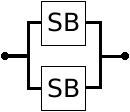
\includegraphics[scale=0.9]{sb_block.png}
  \caption{Reliability block diagram of the system bus subsystem.}
  \label{fig0}
\end{figure}

\subsection{Wheel Unit Model}
Each wheel unit consists of three different components, sensors (S), actuator (A), and computing modules (CM), organized as in \figref{fig2}. There are two redundant CMs, two redundant sensors, and one actuator, yielding the reliability block diagram shown in \figref{fig3}.   
\begin{figure}[H]
  \centering
  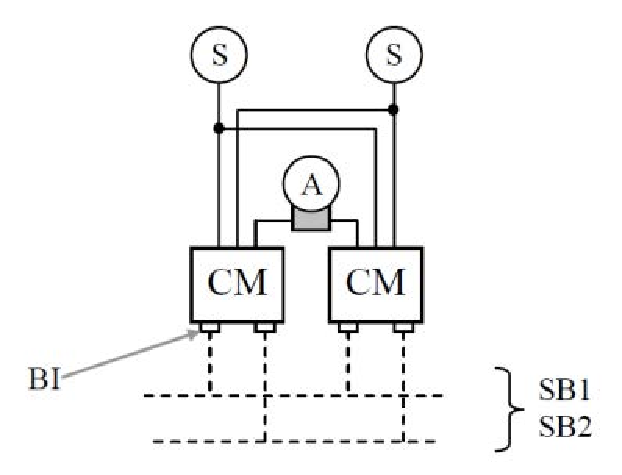
\includegraphics[scale=0.7]{Fig2.pdf}
  \caption{Wheel Unit}
  \label{fig2}
\end{figure}
\begin{figure}[H]
  \centering
  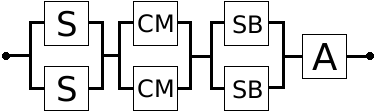
\includegraphics[scale=0.7]{wu_block.png}
  \caption{Reliability block diagram of the wheel unit.}
  \label{fig3}
\end{figure}



%--------------------------------
\subsection{Wheel Unit Subsystem Model}
A combination of four WUs yields the wheel unit subsystem. In the full functionality mode of operation the subsystem can not tolerate any broken WUs, a fault tree in \figref{fig4} is shown for this mode. When running in the other mode of operation, allowing degraded functionality, one WU can become faulty without causing a full system failure, shown in \figref{fig5}. 
\begin{figure}[H]
  \Tree[.{WU Subsystem Failure} [.{$1 \geq$} WU WU WU WU ] ]
  \caption{Fault tree for the Wheel Unit Subsystem, full functionality.}
  \label{fig4}
\end{figure}
\begin{figure}[H]
  \Tree[.{WU Subsystem Failure} [.{$2 \geq$} WU WU WU WU ] ]
  \caption{Fault tree for the Wheel Unit Subsystem, degraded functionality.}
  \label{fig5}
\end{figure}


%--------------------------------
\subsection{Central Unit Model}
In the two evaluated architectures the central unit is configured in two different ways. The distributed architecture's central unit is described in \secref{subsec:dda} and the central unit for the centralized architecture is described in \secref{subsec:cta}. 

\subsubsection{Distributed Duplex Architecture}
\label{subsec:dda}
The distributed architecture's central unit consists of two computing modules (CM) configured in duplex. Each CM fails silent with a coverage factor of $99\%$. If a violation of the fail-silent property occurs, i.e. a CM delivers a erroneous result, the whole central unit fails. In \figref{fig6} the CMs and the serial buses (SB) connecting them, are illustrated. This setup yields the reliability block diagram shown in \figref{fig7}. As the subsystem works like a hot standby system with the failure rates and coverage factor from \tabref{tab:faildist}, the Markov chain model in \figref{fig8} can be derived.

\begin{figure}[H]
  \centering
  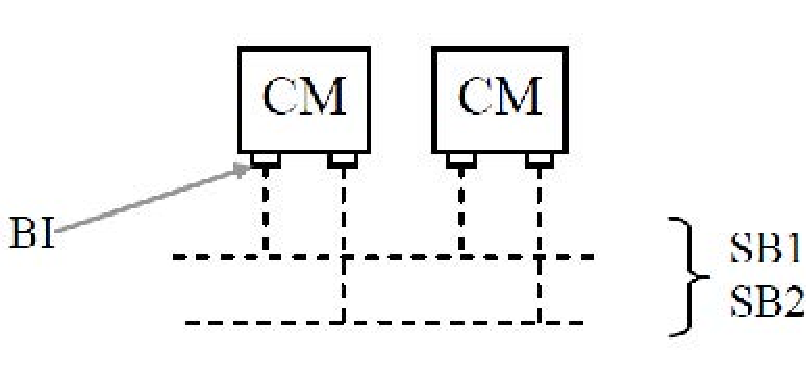
\includegraphics[scale=.5]{Fig6.pdf}
  \caption{Central Unit, duplex configuration.}
  \label{fig6}
\end{figure}
\begin{figure}[H]
  \centering
  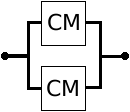
\includegraphics[scale=1.0]{cm2_block.png}
  \caption{Reliability block diagram for the Central Unit, duplex configuration.}
  \label{fig7}
\end{figure}
\begin{figure}[H]
  \begin{center}
    \begin{tikzpicture}[node distance=5mm and 20mm]
      \node[state] (s2) {2};
      \node[state] (s3) [right= of s2] {1};
      \node[state] (s4) [right= of s3] {F};
      \draw [->,bend left=45] (s2) to node[above] {$c*2\lambda_{CU-CM} $} (s3);
      \draw [->,bend right=45] (s2) to node[below] {$(1-c)*2\lambda_{CU-CM}$} (s4);
      \draw [->,bend left=45] (s3) to node[above] {$\lambda_{CU-CM}$} (s4);
    \end{tikzpicture}
  \caption{Markov chain model for central unit with duplex configuration.}
   \label{fig8}
\end{center}
\end{figure}



%-------------
\subsubsection{Centralized Triplex Architecture}
\label{subsec:cta}
For the central unit in the centralized architecture, an additional CM is added making it a triplex configuration instead of duplex. When all three units is working the coverage factor for the first failure is 100\%. This as the three units produce results by majority voting, so even if one unit produces the wrong result, the voting masks it. A module producing an erroneous result is detected by the other modules and is shutdown. When this happens, the system reconfigures into a duplex system. 

How the CMs are connected can be seen in \figref{fig9}, and the corresponding reliability block diagram in \figref{fig10}. From the Markov chain model in \figref{fig11} it is easy to see that when the first unit fails, and a transition from state 3 to state 2 is made, the system behaves the same as the duplex configuration described in \secref{subsec:dda}. 

\begin{figure}[H]
  \centering
  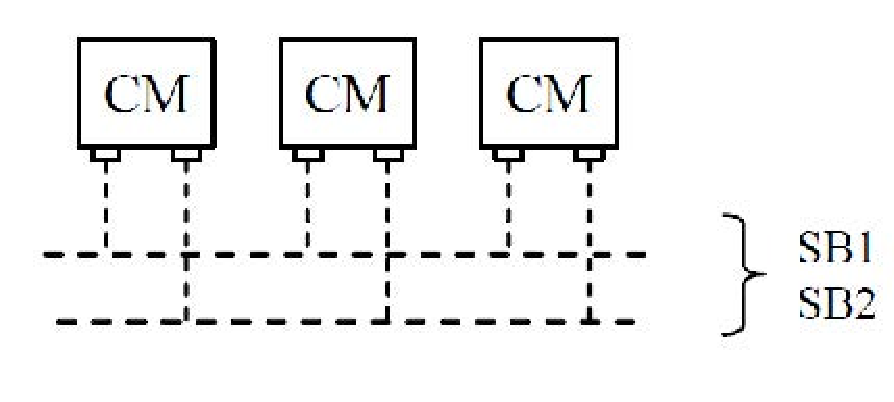
\includegraphics[scale=.5]{Fig9.pdf}
  \caption{Central Unit, triplex configuration.}
  \label{fig9}
\end{figure}

\begin{figure}[H]
  \centering
  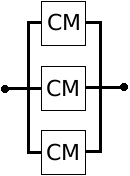
\includegraphics[scale=1.0]{cm3_block.png}
  \caption{Reliability block diagram for central unit in triplex configuration.}
  \label{fig10}
\end{figure}
\begin{figure}[H]
  \centering
  \begin{tikzpicture}[node distance=5mm and 20mm]
    \node[state] (sa) {3};
    \node[state] (sb) [right= of sa] {2};
    \node[state] (sc) [right= of sb] {1};
    \node[state] (sd) [right= of sc] {F};
    \draw [->,bend left=45] (sa) to node[above] {$3\lambda_{CU-CM} $} (sb);
    \draw [->,bend left=45] (sb) to node[above] {$c*2\lambda_{CU-CM} $} (sc);
    \draw [->,bend right=45] (sb) to node[below] {$(1-c)*2\lambda_{CU-CM}$} (sd);
    \draw [->,bend left=45] (sc) to node[above] {$\lambda_{CU-CM}$} (sd);
  \end{tikzpicture}
  \caption{Markov chain model for central unit in triplex configuration.}
  \label{fig11}
\end{figure}





%--------------------------------
\subsection{System Model}
Here models for the two different system architectures and their modes of operation are described.

\subsubsection{Centralized Architecture}
\label{subsubsec:smca}
In \figref{fig12} a fault tree for the centralized architecture, running in the full functionality mode of operation, is displayed, and a fault tree for the degraded functionality is shown in \figref{fig13}. In both modes of operation it is clear from the fault trees that the system will still be working with two broken CMs and one broken SB, but for the degraded functionality mode of operation the system can handle one broken wheel unit, which the other mode can not.    

\begin{figure}[H]
  \Tree[.{System Failure} [.{$1 \geq$} [.{CU subsystem fail} [.{$\&$} CM CM CM ] ] [.{WU subsystem fail} [.{$1 \geq$} WU WU WU WU ] ] [.{SB subsystem fail} [.{\&} SB SB ] ] ] ]
  \caption{Fault tree for Full Functionality.}
  \label{fig12}
\end{figure}
\begin{figure}[H]
  \Tree[.{System Failure} [.{$1 \geq$} [.{CU subsystem fail} [.{$\&$} CM CM CM ] ] [.{WU subsystem fail} [.{$2 \geq$} WU WU WU WU ] ] [.{SB subsystem fail} [.{\&} SB SB ] ] ] ]
  \caption{Fault tree for Degraded Functionality.}
  \label{fig13}
\end{figure}

%-------------
\subsubsection{Distributed Architecture}
For the distributed architecture, fault trees for full functionality and degraded functionality is shown in \figref{fig14} and \figref{fig15}, respectively. The difference between them is the same as in \secref{subsubsec:smca}, with the exception that in this architecture, the system can only handle one broken CM before failing.

\begin{figure}[H]
  \Tree[.{System Failure} [.{$1 \geq$} [.{CU subsystem fail} [.{$\&$} CM CM ] ] [.{WU subsystem fail} [.{$1 \geq$} WU WU WU WU ] ] [.{SB subsystem fail} [.{\&} SB SB ] ] ] ]
  \caption{Fault tree for Full Functionality.}
  \label{fig14}
\end{figure}
\begin{figure}[H]
  \Tree[.{System Failure} [.{$1 \geq$} [.{CU subsystem fail} [.{$\&$} CM CM ] ] [.{WU subsystem fail} [.{$2 \geq$} WU WU WU WU ] ] [.{SB subsystem fail} [.{\&} SB SB ] ] ] ]
  \caption{Fault tree for Degraded Functionality.}
  \label{fig15}
\end{figure}